% Classical Pesaran GVAR — what it does. Standalone TikZ -> PDF -> PNG.
\documentclass[border=10pt]{standalone}
\usepackage[T1]{fontenc}
\usepackage{helvet}
\renewcommand{\familydefault}{\sfdefault}
\usepackage{amsmath,amssymb,bm}
\usepackage{tikz}
\usetikzlibrary{arrows.meta,positioning,calc,shapes.geometric,fit,backgrounds}

\definecolor{MadridBlue}{RGB}{28,54,99}
\definecolor{MadridBlue2}{RGB}{48,91,150}
\definecolor{Ink}{RGB}{35,35,35}
\definecolor{Muted}{RGB}{105,105,105}
\definecolor{LightGrey}{RGB}{244,245,247}
\definecolor{MidGrey}{RGB}{210,214,221}
\definecolor{SoftBlue}{RGB}{235,241,249}
\definecolor{SoftBlue2}{RGB}{224,233,246}
\definecolor{AccentRed}{RGB}{150,45,45}
\definecolor{CheckGreen}{RGB}{39,116,75}

\tikzset{
  ctry/.style={rounded corners=3pt, draw=MadridBlue, line width=0.8pt, fill=SoftBlue,
    text=Ink, align=center, inner sep=5pt, font=\footnotesize, minimum height=1.55cm, text width=2.75cm},
  usbox/.style={ctry, fill=MadridBlue, text=white, draw=MadridBlue, line width=1.1pt},
  proc/.style={rounded corners=3pt, draw=MadridBlue, line width=0.9pt, fill=LightGrey,
    text=Ink, align=center, inner sep=7pt, font=\small},
  solve/.style={proc, fill=SoftBlue, draw=MadridBlue, line width=1.4pt},
  note/.style={align=left, font=\scriptsize, text=Muted, inner sep=2pt},
  redtag/.style={rounded corners=2pt, draw=AccentRed, line width=0.7pt, fill=white,
    text=AccentRed, align=center, font=\scriptsize\bfseries, inner sep=3pt},
  flowarr/.style={-{Stealth[length=2.6mm]}, draw=MadridBlue2, line width=1.0pt},
  linkarr/.style={{Stealth[length=2mm]}-{Stealth[length=2mm]}, draw=Muted, line width=0.7pt, dashed},
}

\begin{document}
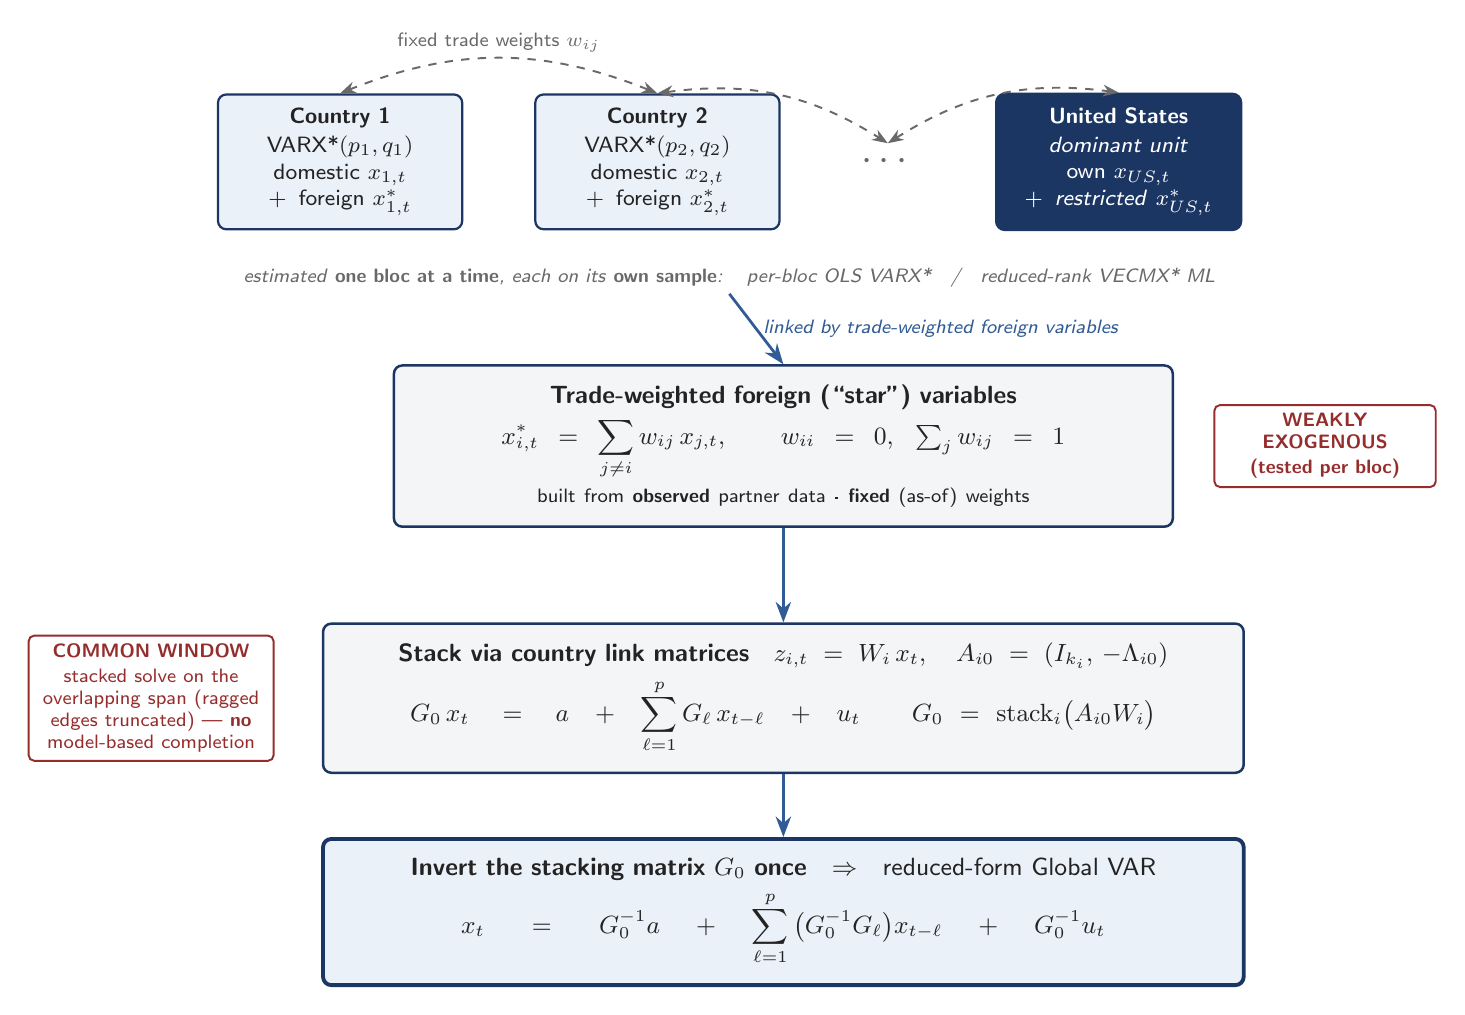
\begin{tikzpicture}

% ---------------- country model row ----------------
\node[ctry] (c1) {\textbf{Country 1}\\[1pt]VARX*$(p_1,q_1)$\\ domestic $x_{1,t}$\\ +\, foreign $x^*_{1,t}$};
\node[ctry, right=9mm of c1] (c2) {\textbf{Country 2}\\[1pt]VARX*$(p_2,q_2)$\\ domestic $x_{2,t}$\\ +\, foreign $x^*_{2,t}$};
\node[right=9mm of c2, font=\Large\bfseries, text=Muted] (dots) {$\cdots$};
\node[usbox, right=9mm of dots] (cus) {\textbf{United States}\\[1pt]\emph{dominant unit}\\ own $x_{US,t}$\\ +\, \emph{restricted} $x^*_{US,t}$};

% cross-country fixed-weight links (dashed) among the separate models
\draw[linkarr] (c1.north) to[bend left=22] node[above,note,text=Muted]{fixed trade weights $w_{ij}$} (c2.north);
\draw[linkarr] (c2.north) to[bend left=20] (dots.north);
\draw[linkarr] (dots.north) to[bend left=20] (cus.north);
% US is a source, not a receiver (financial stars restricted) — marked on the box itself.

% estimation label centred just below the row; the main flow starts from here
\node[note, text=Muted, font=\scriptsize\itshape, anchor=north] (estlab)
  at ($(c1.south)!0.5!(cus.south)+(0,-0.4)$)
  {estimated \textbf{one bloc at a time}, each on its \textbf{own sample}: \; per-bloc OLS VARX* \; / \; reduced-rank VECMX* ML};

% ---------------- foreign-star construction strip ----------------
\node[proc, below=1.7cm of c2, xshift=1.6cm, text width=9.4cm, fill=LightGrey] (stars)
  {\textbf{Trade-weighted foreign (``star'') variables}\\[2pt]
   $\displaystyle x^*_{i,t}=\sum_{j\neq i} w_{ij}\,x_{j,t},\qquad w_{ii}=0,\ \ \textstyle\sum_j w_{ij}=1$\\[2pt]
   {\scriptsize built from \textbf{observed} partner data · \textbf{fixed} (as-of) weights}};
\node[redtag, right=5mm of stars.east, text width=2.6cm] (we)
  {WEAKLY\\ EXOGENOUS\\[1pt]\scriptsize(tested per bloc)};

\draw[flowarr] (estlab.south) -- node[right,note,text=MadridBlue2,font=\scriptsize\itshape,pos=0.5]{linked by trade-weighted foreign variables} (stars.north);

% ---------------- stacking + single inversion ----------------
\node[proc, below=1.2cm of stars, text width=11.2cm] (stack)
  {\textbf{Stack via country link matrices} \; $z_{i,t}=W_i\,x_t,\quad A_{i0}=(I_{k_i},\,-\Lambda_{i0})$\\[3pt]
   $\displaystyle G_0\,x_t \;=\; a \;+\; \sum_{\ell=1}^{p} G_\ell\,x_{t-\ell} \;+\; u_t
      \qquad G_0=\operatorname{stack}_i\!\big(A_{i0}W_i\big)$};

\node[solve, below=8mm of stack, text width=11.2cm] (solve)
  {\textbf{Invert the stacking matrix} $G_0$ \textbf{once} $\;\Rightarrow\;$ reduced-form Global VAR\\[3pt]
   $\displaystyle x_t \;=\; G_0^{-1}a \;+\; \sum_{\ell=1}^{p}\big(G_0^{-1}G_\ell\big)x_{t-\ell} \;+\; G_0^{-1}u_t$};

\draw[flowarr] (stars.south) -- (stack.north);
\draw[flowarr] (stack.south) -- (solve.north);

% ---------------- red side callout: common solve window ----------------
\node[redtag, left=6mm of stack.west, text width=2.9cm, anchor=east] (bp)
  {COMMON WINDOW\\[1pt]\scriptsize\mdseries stacked solve on the overlapping span (ragged edges truncated) — \textbf{no} model-based completion};

\end{tikzpicture}
\end{document}
